%\documentclass[a4paper]{article}
%\usepackage{beamerarticle}
%\documentclass[handout]{beamer}
%\usepackage{handoutWithNotes}
%\setbeameroption{show notes} 
%\pgfpagesuselayout{4 on 1 with notes}[a4paper,border shrink=5mm]
%\documentclass[ignorenonframetext,red]{beamer}

%\documentclass[notes=only]{beamer} %notes only
% \documentclass[notes]{beamer} %slides with notes
\documentclass{beamer}

\mode<presentation>{
	% \usetheme{Goettingen}
	\usetheme{CambridgeUS} 
	\usecolortheme{beaver}
	%\setbeamercovered{transparent}
}

%set up chinese environment
\usepackage{fontspec}
\newfontfamily\zhfont[BoldFont=Hiragino Sans GB W3]{Hiragino Sans GB W3} %设置中文
\newfontfamily\zhpunctfont{Hiragino Sans GB W3} % 设置中文
\XeTeXlinebreaklocale "zh"
\XeTeXlinebreakskip = 0pt plus 1pt
\renewcommand{\today}{\number\year 年\number\month 月\number\day 日}
% \setmainfont{Hiragino Sans GB W3}           %这里设置英文衬线字体
% \setmonofont{Hiragino Sans GB W3}                     %英文等宽字体
% \setsansfont{Hiragino Sans GB W3}               %英文无衬线字体
\usepackage{zhspacing}
\zhspacing

% set up other environment
\usepackage[english]{babel}
\usepackage[utf8]{inputenc}
\usepackage{graphicx}
\usepackage{times}
\usepackage[T1]{fontenc}
\usepackage{animate}
% \usepackage[caption=false,font=footnotesize]{subfig}
\usepackage[font=footnotesize]{subfig}
\usepackage{listings}
\lstset{language=C++}
\lstset{breaklines}
\lstset{extendedchars=false}
\lstset{basicstyle=\tiny}
\lstset{frame=shadowbox}

\usepackage[justification = centering,
labelsep = period,font = scriptsize]{caption}
\setlength{\abovecaptionskip}{1pt}
\setlength{\belowcaptionskip}{1pt}
\usepackage{amssymb}
\usepackage{epstopdf}
%tikz packages
\usepackage{tikz}
\usetikzlibrary{mindmap,trees}

\setbeamertemplate{footline}[frame number]

\title{基于Intel Xeon/Xeon Phi平台的关于离散时间对冲误差的并行化研究}

\logo{
  
\includegraphics[width=0.4cm,height=0.4cm,keepaspectratio]{Figures/logo-MdS.jpg}%
  \hspace{0.5ex}
  
\includegraphics[width=0.4cm,height=0.4cm,keepaspectratio]{Figures/logo-CEA.jpg}%
  \hspace{0.5ex}
  
\includegraphics[width=0.6cm,height=0.8cm,keepaspectratio]{Figures/logo-cnrs2.png}%
  \hspace{0.5ex}
  
\includegraphics[width=0.4cm,height=0.35cm,keepaspectratio]{Figures/logo-versaille2.png}%
}

\institute[机构1,机构2, 机构3] % (optional, but mostly needed)
{
  \inst{1} Maison de la Simulation 
  \and
  \inst{2} Atomic Energy and Alternative Energies Commission (C.E.A) 
  \and
  \inst{3} French National Centre for Scientific Research (C.N.R.S) 
  \and
  \inst{4} Versailles Saint-Quentin-en-Yvelines University \\ 
  \vspace{3ex}
  \scalebox{4}{\insertlogo}
}

\author[作者] % (optional, use only with lots of authors)
{\scriptsize 叶帆\inst{1,2} \and 陈浪石\inst{1,3} \and 潘慈辉\inst{1,4}}

% % - Keep it simple, no one is interested in your street address.
%
% \only<presentation>{
%
%   \subject{Krylov Subspace, Auto-tuning, Arnoldi Orthogonalization}
% }

% \pgfdeclareimage[height=0.5cm]{university-logo}{university-logo-filename}
% \logo{\pgfuseimage{university-logo}}

% Delete this, if you do not want the table of contents to pop up at
% the beginning of each subsection:

\AtBeginSection[]
{
	\begin{withoutheadline}
		\begin{frame}<beamer>{内容提要}
			\tableofcontents[currentsection,currentsubsection]
		\end{frame}
	\end{withoutheadline}
}

% If you wish to uncover everything in a step-wise fashion, uncomment
% the following command: 
%\beamerdefaultoverlayspecification{<+->}

\makeatletter
\newenvironment{withoutheadline}{
  \setbeamertemplate{headline}[default]
  \def\beamer@entrycode{\vspace*{-\headheight}}
}{}
\makeatother
\setbeamertemplate{navigation symbols}{}
\setbeamertemplate{footline}[pagenumber]

\begin{document}

\begin{frame}[plain]
	\titlepage
\end{frame}

%remove logs at footline of each page
\setbeamertemplate{logo}{}

\begin{withoutheadline}
\begin{frame}
	\frametitle{内容提要}
	% \tableofcontents[hideothersubsections]
	\tableofcontents
	\note[item]{注释说明1}
\end{frame}
\end{withoutheadline}

\section{背景介绍} % (fold)
\label{sec:context}

\begin{withoutheadline}
\begin{frame}
	\frametitle{超算发展及Xeon Phi}
	\begin{columns}
		\column{0.4\textwidth}
			高性能计算已经进入后Petaflop($10^{15}$)时代。但是能优化到Petaflop级别的实际应用却很少,面临问题如下
			\vspace{1ex}
			\begin{itemize}
				\item 算法的内在并行性不足
				\vspace{1ex}
				\item 并行算法的通信受制于内存和网络连接
				\vspace{1ex}
				\item 并行编程的难度
			\end{itemize}
			\vspace{1ex}
			超级计算机本身还面临
			\begin{itemize}
				\item 能耗过大
			\end{itemize}
		\column{0.6\textwidth}
			\begin{figure}[htbp]
				\centering
				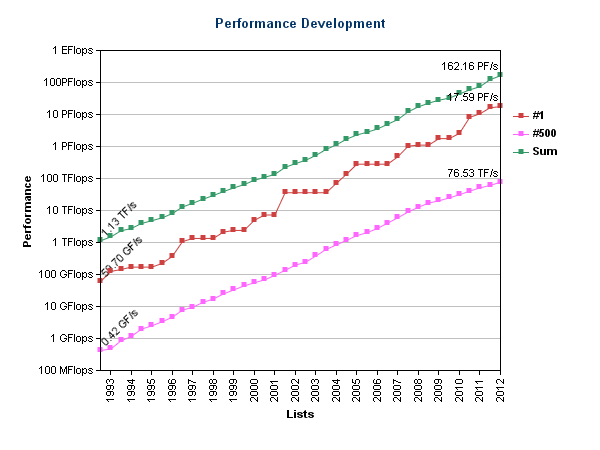
\includegraphics[width=\textwidth]{Figures/context/top500Perf.png}
				\caption{超算Top500发展趋势}
				\label{fig:top500}
			\end{figure}
	\end{columns}
\end{frame}
\end{withoutheadline}

\begin{withoutheadline}
\begin{frame}
	\frametitle{超算发展及Xeon Phi}
	\begin{columns}
		\column{0.4\textwidth}
			单个CPU的发展已经达到性能和功耗的瓶颈,超算转向众核架构(Manycore), 其具有如下优势
			\begin{itemize}
				\item 高带宽(bandwidth)带来的高通量(high data throughput)
				\item 高能耗效率(flops/watt)
					\note[item]{世界绿色500强榜单上的高能效机器越来越多采用众核结构}
				\item 适合大规模的数据并行性应用(data parallel)
			\end{itemize}
			目前众核结构处理器的代表
			\begin{itemize}
				\item Nvidia 的GPU加速器
				\item Intel 的Xeon Phi协处理器
			\end{itemize}
		\column{0.6\textwidth}
		\begin{figure}[htbp]
			\centering
			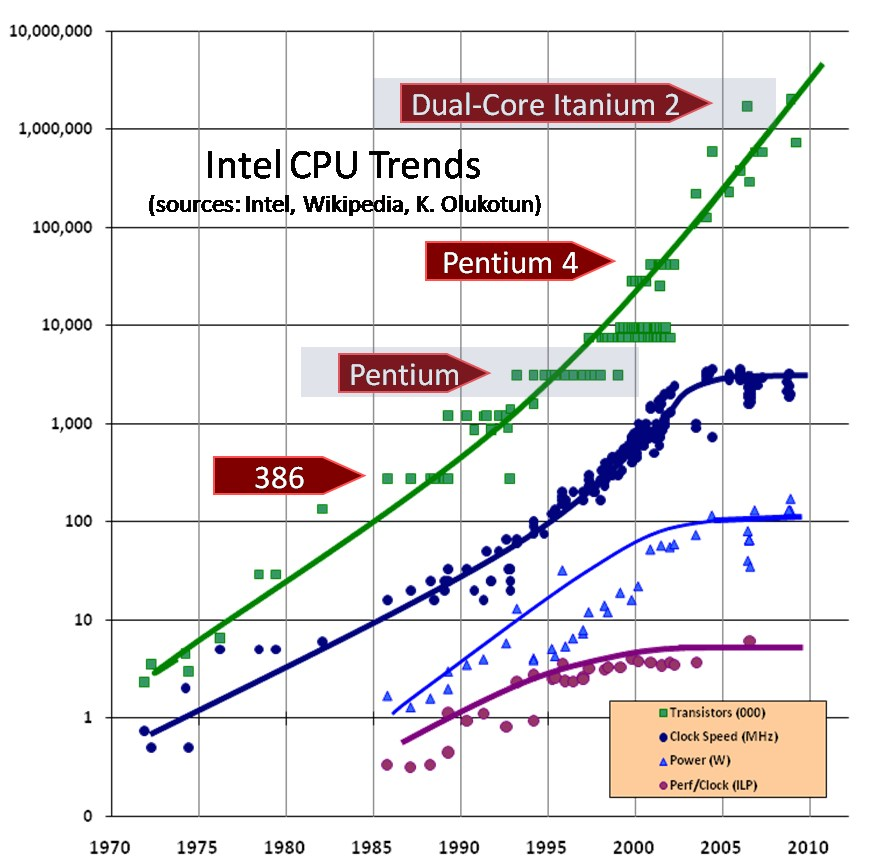
\includegraphics[width=0.8\textwidth]{Figures/context/CPU-Scaling.jpg}
			\caption{单个CPU发展遇到的各种瓶颈问题}
			\label{fig:CPUScale}
		\end{figure}
	\end{columns}
\end{frame}
\end{withoutheadline}

\begin{withoutheadline}
	\begin{frame}
		\frametitle{金融领域的超算}
		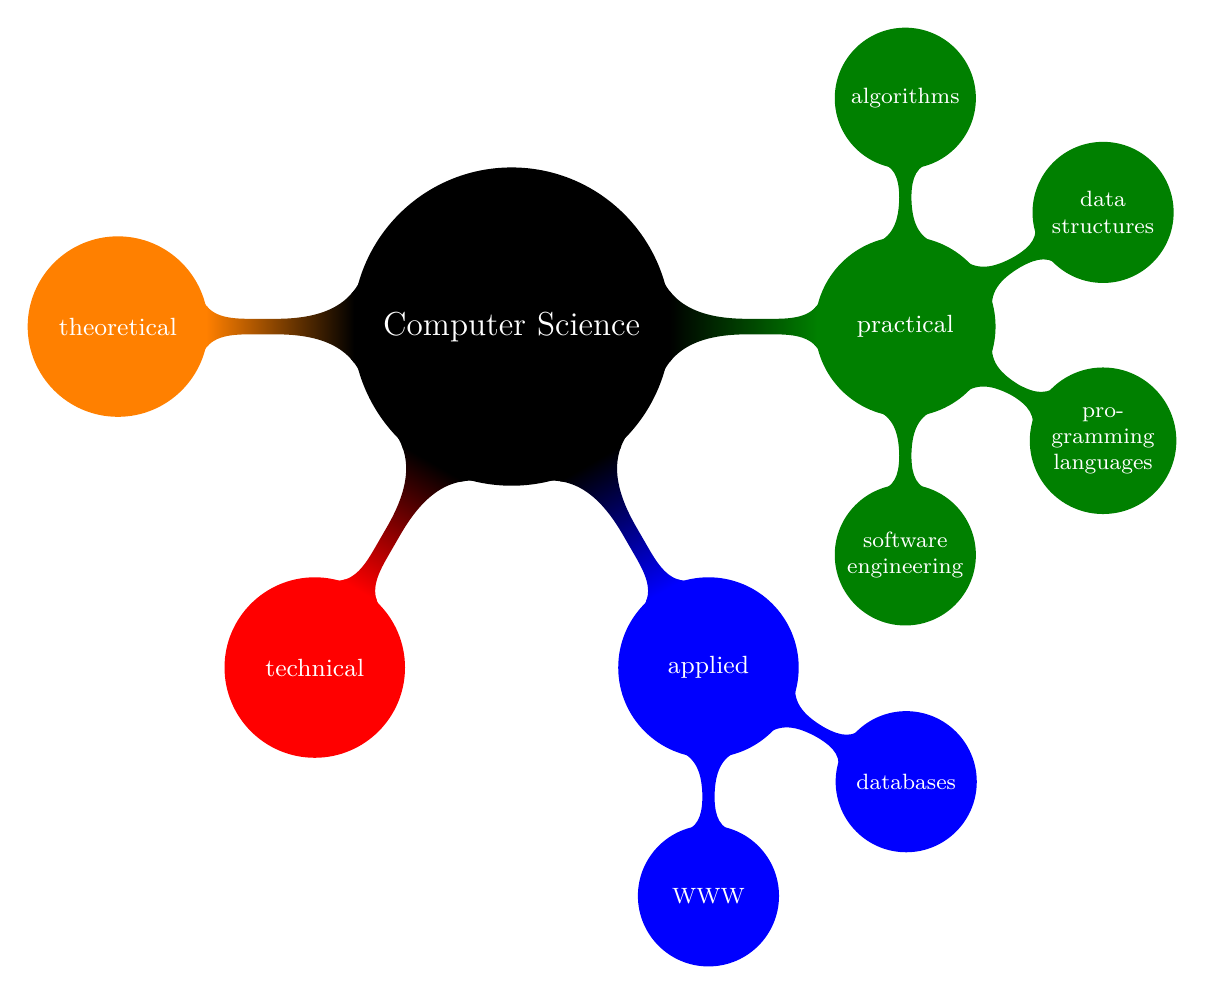
\begin{tikzpicture}
			\path[mindmap,concept color=black,text=white]
			node[concept] {Computer Science}
			[clockwise from=0]
			child[concept color=green!50!black] {
				node[concept] {practical}
				[clockwise from=90]
				child { node[concept] {algorithms} }
				child { node[concept] {data structures} }
				child { node[concept] {pro\-gramming languages} }
				child { node[concept] {software engineer\-ing} }
			}  
			child[concept color=blue] {
				node[concept] {applied}
				[clockwise from=-30]
				child { node[concept] {databases} }
				child { node[concept] {WWW} }
			}
			child[concept color=red] { node[concept] {technical} }
			child[concept color=orange] { node[concept] {theoretical} };
		\end{tikzpicture}
	\end{frame}
\end{withoutheadline}

% section 背景介绍 (end)

\section{课题陈述} % (fold)
\label{sec:subject}

\begin{withoutheadline}
\begin{frame}
	\frametitle{欧式期权}
	content	
\end{frame}
\end{withoutheadline}

\begin{withoutheadline}
\begin{frame}
	\frametitle{Black-Scholes模型}
	content
\end{frame}
\end{withoutheadline}

\begin{withoutheadline}
\begin{frame}
	\frametitle{对冲策略及误差分析}
	content
\end{frame}
\end{withoutheadline}
% section 课题陈述 (end)

\begin{withoutheadline}
\begin{frame}
	\frametitle{参数选择及收敛条件}
	content	
\end{frame}
\end{withoutheadline}

\section{并行化算法} % (fold)
\label{sec:algorithm}

\begin{withoutheadline}
\begin{frame}
	\frametitle{并行性分析}
	content	
\end{frame}
\end{withoutheadline}

\begin{withoutheadline}
\begin{frame}
	\frametitle{单MIC并行优化}
	content	
\end{frame}
\end{withoutheadline}

\begin{withoutheadline}
\begin{frame}
	\frametitle{基于汇编的矢量化积分运算}
	content	
\end{frame}
\end{withoutheadline}

\begin{withoutheadline}
\begin{frame}
	\frametitle{N值的最优化搜索}
	content	
\end{frame}
\end{withoutheadline}

\begin{withoutheadline}
\begin{frame}
	\frametitle{多MIC并行优化}
	content	
\end{frame}
\end{withoutheadline}

% section 并行化算法 (end)

\section{实验结果及分析} % (fold)
\label{sec:exp}

\begin{withoutheadline}
\begin{frame}
	\frametitle{单MIC及CPU版本的实验对比}
	content	
\end{frame}
\end{withoutheadline}

\begin{withoutheadline}
\begin{frame}
	\frametitle{多MIC优化实验及结果分析}
	content	
\end{frame}
\end{withoutheadline}

\begin{withoutheadline}
\begin{frame}
	\frametitle{算法的收敛性研究}
	content	
\end{frame}
\end{withoutheadline}

% section 实验结果及分析 (end)

\begin{withoutheadline}
  \begin{frame}{参考文献}
	\scriptsize
	\bibliographystyle{splncs}
	\bibliography{docear}
  \end{frame}
\end{withoutheadline}

\end{document}
